% =====================================================================
%  Cinema Seat Reservation - Final Presentation Slides (Beamer)
%  15 slides matching the coursework submission.
%  Compile with: pdflatex slides.tex   (run twice)
% =====================================================================
\documentclass[aspectratio=169,11pt]{beamer}

% ---------- theme & colour ----------
\usetheme{Madrid}
\usecolortheme{whale}

\definecolor{primary}{RGB}{0,51,102}
\definecolor{accent}{RGB}{0,102,153}
\definecolor{lightbg}{RGB}{245,246,248}

\setbeamercolor{structure}{fg=primary}
\setbeamercolor{frametitle}{fg=white,bg=primary}
\setbeamercolor{title}{fg=primary}
\setbeamercolor{subtitle}{fg=accent}
\setbeamercolor{block title}{bg=primary,fg=white}
\setbeamercolor{block body}{bg=primary!8}
\setbeamercolor{item}{fg=accent}
\setbeamertemplate{navigation symbols}{}

% ---------- fonts & layout ----------
\usepackage[utf8]{inputenc}
\usepackage[T1]{fontenc}
\usepackage{lmodern}
\usepackage{microtype}
\usepackage{booktabs}
\usepackage{tabularx}
\usepackage{array}
\usepackage{graphicx}
\usepackage{amssymb}
\usepackage{pifont}
\usepackage{tikz}
\usetikzlibrary{arrows.meta,positioning}
\usepackage{listings}

\newcommand{\code}[1]{\texttt{#1}}

% ---------- header / footer ----------
\setbeamertemplate{footline}{%
  \leavevmode%
  \hbox{%
    \begin{beamercolorbox}[wd=0.5\paperwidth,ht=2.5ex,dp=1ex,left]{author in head/foot}%
      \hspace*{1ex}\tiny Cinema Seat Reservation
    \end{beamercolorbox}%
    \begin{beamercolorbox}[wd=0.5\paperwidth,ht=2.5ex,dp=1ex,right]{date in head/foot}%
      \tiny Group Coursework \hspace*{1ex}\insertframenumber/\inserttotalframenumber\hspace*{1ex}
    \end{beamercolorbox}}%
  \vskip0pt}

% =====================================================================
\begin{document}

% =====================================================================
%  SLIDE 1 - Title, domain, members
% =====================================================================
\begin{frame}[plain]
  \centering
  \vspace{0.35cm}
  {\Huge\color{primary}\textbf{Cinema Seat Reservation}}\\[0.3cm]
  {\large\color{accent} Domain-Driven Design, Test-Driven Development
  and Clean Architecture}\\[0.4cm]
  {\small DOMAIN: Cinema Seat Reservation}\\[1.1cm]

  \begin{center}
  \begin{tabularx}{0.82\textwidth}{@{}l X l@{}}
    \toprule
    \textbf{Name} & \textbf{Role} & \textbf{Reg. No.} \\
    \midrule
    BYAMUGISHA ANTHONY & Domain Lead & 24/U/0360 \\
    AKELLO BEATRICE & Domain Model Lead & 24/U/25856/EVE \\
    NDAWULA HABIBAH & Architecture Lead & 24/U/10049/EVE \\
    MENHYA JOSHUA KIBEDI & Integration Lead & 24/U/06798/EVE \\
    All members (shared) & Testing & --- \\
    \bottomrule
  \end{tabularx}
  \end{center}

  \vspace{0.7cm}
  {\small \textbf{Dept. of Networks} ~•~ School of Computing and
  Informatics Technology, Makerere University}\\
  {\small \textbf{Instructor:} Kasozi W. Vincent}\\[0.35cm]
  {\footnotesize \code{https://github.com/anthonybyamugisha/Cinema-Seat-Reservation}}\\[0.25cm]
  {\footnotesize Small Domain ~•~ Explicit Business Rules ~•~ Traceable Design ~•~ Executable Tests}
\end{frame}

% =====================================================================
%  SLIDE 2 - Problem, scope, exclusions, terms
% =====================================================================
\begin{frame}{Problem, Scope, Exclusions \& Key Terms}
  \textbf{Problem.} Cinema customers need to reserve a specific seat for a
  particular show, and the same seat must never be allocated to more than one
  reservation for that show. The system coordinates reservation confirmation
  with the show's seat inventory, preserving valid reservation states and
  seat-allocation rules.

  \begin{columns}[t]
    \begin{column}{0.49\textwidth}
      \begin{block}{Inside our scope}
        \footnotesize
        \begin{itemize}
          \item Confirm an existing reservation (use case 1)
          \item Reserve the seat in the Show (use case 2)
          \item Validate seat numbers; check eligibility
          \item Enforce reservation state transitions
          \item Prevent double seat allocation
          \item Raise/handle \code{ReservationConfirmed} event
          \item In-memory repositories; success/failure result
        \end{itemize}
      \end{block}
    \end{column}
    \begin{column}{0.49\textwidth}
      \begin{block}{Exclusions}
        \footnotesize
        \begin{itemize}
          \item Payments, pricing, auth, refunds/cancellations
          \item Ticket printing, recommendations, notifications
          \item Venue-map design, concurrency/locking
          \item Production database, web/mobile UI
          \item Deployment, microservices, message brokers
          \item Creating reservations and shows
        \end{itemize}
      \end{block}
    \end{column}
  \end{columns}

  \vspace{0.15cm}
  \scriptsize
  \textbf{Key terms:}
  \textbf{Reservation} (seat request, PENDING$\rightarrow$CONFIRMED) \;
  \textbf{Show} (screening with start time + seat inventory) \;
  \textbf{ShowSeat} (a seat in a Show, AVAILABLE/RESERVED) \;
  \textbf{SeatNumber} (row A--Z + position 1--50) \;
  \textbf{ReservationConfirmed} (domain event requesting seat allocation).
\end{frame}

% =====================================================================
%  SLIDE 3 - Business rules BR1-BR6
% =====================================================================
\begin{frame}{Business Rules BR1--BR6}
  \centering
  \scriptsize
  \begin{tabularx}{\textwidth}{@{}c c X X@{}}
    \toprule
    \textbf{BR} & \textbf{Rule type} & \textbf{Rule statement} &
    \textbf{Responsible component; Violation outcome} \\
    \midrule
    BR1 & Value &
      SeatNumber = one row letter A--Z + position 1--50 &
      \code{SeatNumber} VO; \code{InvalidSeatNumberError} \\
    BR2 & Identity/state &
      Reservation starts PENDING; only PENDING may become CONFIRMED &
      \code{Reservation} Aggregate Root; \code{InvalidReservationStateError} \\
    BR3 & Invariant &
      In one Show, a ShowSeat may be allocated to at most one Reservation &
      \code{Show} Aggregate Root; \code{SeatAlreadyReservedError} \\
    BR4 & Cross-concept &
      Eligible only if Show has not started AND customer has $<$ 4 confirmed
      seats in that Show &
      \code{ReservationEligibilityService} (Domain Service);
      \code{ReservationNotEligibleError} \\
    BR5 & Follow-up &
      On confirmation, reservation raises \code{ReservationConfirmed} which
      requests the Show to reserve the seat &
      \code{Reservation} raises; \code{ReservationConfirmedHandler};
      if Show rejects, nothing is saved, reservation stays PENDING \\
    BR6 & Lookup &
      Reservation must be retrieved from repository before confirmation &
      \code{ConfirmReservationService} + \code{ReservationRepository};
      \code{ReservationNotFoundError} \\
    \bottomrule
  \end{tabularx}

  \vspace{0.3cm}
  {\scriptsize Each rule = rule statement + responsible component + violation
  outcome. All six rule types required by the assignment are covered.}
\end{frame}

% =====================================================================
%  SLIDE 4 - Value objects and entities
% =====================================================================
\begin{frame}{Value Object and Entity Choices}
  \begin{columns}[t]
    \begin{column}{0.33\textwidth}
      \begin{block}{SeatNumber --- Value Object (BR1)}
        \footnotesize
        \begin{itemize}
          \item Seat identifier such as \code{A10}
          \item No independent identity
          \item Defined by row + position, compared by value
          \item Immutable; validates itself on creation
          \item \code{A10} valid $|$ \code{A51} invalid
        \end{itemize}
        {\scriptsize\itshape Identity is the value itself.}
      \end{block}
    \end{column}
    \begin{column}{0.33\textwidth}
      \begin{block}{Reservation --- Entity / Root (BR2)}
        \footnotesize
        \begin{itemize}
          \item Identity: \code{reservation\_id} (e.g. \code{R001})
          \item Identity persists through state changes
          \item Business lifecycle: PENDING $\rightarrow$ CONFIRMED
          \item Controls its own transitions via \code{confirm()}
          \item Violation: \code{InvalidReservationState}
        \end{itemize}
      \end{block}
    \end{column}
    \begin{column}{0.33\textwidth}
      \begin{block}{ShowSeat --- Child Entity (BR3)}
        \footnotesize
        \begin{itemize}
          \item Identity: \code{seat\_number} within a Show
          \item Changing state: AVAILABLE $\rightarrow$ RESERVED
          \item S001/A10 $\neq$ S002/A10 (same number, different Shows)
          \item Lives inside the Show aggregate only
        \end{itemize}
      \end{block}
    \end{column}
  \end{columns}

  \vspace{0.15cm}
  {\scriptsize BR1 $\rightarrow$ SeatNumber is modelled by value; BR2 $\rightarrow$
  Reservation is modelled by identity and lifecycle.}
\end{frame}

% =====================================================================
%  SLIDE 5 - Aggregates and invariants
% =====================================================================
\begin{frame}{Aggregates and Invariants}
  \begin{columns}[t]
    \begin{column}{0.5\textwidth}
      \begin{block}{Aggregate A --- Reservation}
        \scriptsize
        \begin{itemize}
          \item \textbf{Root:} Reservation
          \item Contains: reservation\_id, customer\_id, show\_id,
                seat\_number, status, domain events
          \item \textbf{Invariant (BR2):} may transition PENDING $\rightarrow$
                CONFIRMED only once, via its own behaviour
          \item Controlled behaviour: \code{Reservation.confirm()}
        \end{itemize}
      \end{block}
    \end{column}
    \begin{column}{0.5\textwidth}
      \begin{block}{Aggregate B --- Show}
        \scriptsize
        \begin{itemize}
          \item \textbf{Root:} Show
          \item Contains: show\_id, start\_time, collection of ShowSeats
          \item \textbf{Invariant (BR3):} one SeatNumber may be allocated to
                at most one Reservation
          \item Controlled behaviour: \code{Show.reserve\_seat()}
          \item \code{A10: AVAILABLE} $\rightarrow$ \code{RESERVED by R001} \checkmark \\
                \code{A10: RESERVED by R001} $\rightarrow$ \code{R002} \ding{55}
        \end{itemize}
      \end{block}
    \end{column}
  \end{columns}

  \vspace{0.15cm}
  {\scriptsize Aggregates never hold references to each other --- communication
  happens only through the BR5 domain event. \textbf{Reservation} protects
  lifecycle consistency; \textbf{Show} protects the no-double-allocation
  invariant of its seat inventory.}
\end{frame}

% =====================================================================
%  SLIDE 6 - Domain service and factory (CORRECTED)
% =====================================================================
\begin{frame}{Domain Service (BR4) and Factory Decision}
  \begin{columns}[t]
    \begin{column}{0.5\textwidth}
      \begin{block}{ReservationEligibilityService --- Domain Service}
        \scriptsize
        \begin{itemize}
          \item \textbf{Enforces BR4} (cross-concept rule)
          \item Needs info from several concepts: Show start time, Customer,
                existing confirmed reservations in that Show, current time
          \item Does not belong naturally to one entity $\Rightarrow$ Domain
                Service
          \item Stateless, zero collaborators; takes
                \code{(reservation, show, current\_time)}
          \item Violation: \code{ReservationNotEligible}, no event raised
        \end{itemize}
        {\scriptsize\itshape Application coordinates; Domain decides.}
      \end{block}
    \end{column}
    \begin{column}{0.5\textwidth}
      \begin{block}{Factory Decision}
        \scriptsize
        \begin{itemize}
          \item \textbf{Used for \code{Show.create()} only}
          \item Building the full seat map --- every row exists, every seat
                starts AVAILABLE --- is a construction rule
          \item Centralises creation; prevents invalid Shows
          \item \textbf{Not used} for Reservation: the constructor already
                fully describes it
          \item Adding a factory without a reason would add indirection
        \end{itemize}
      \end{block}
    \end{column}
  \end{columns}

  \vspace{0.12cm}
  {\scriptsize BR4 lives in a Domain Service because it spans multiple concepts;
  the Factory is limited to Show because only Show creation has real rules.}
\end{frame}

% =====================================================================
%  SLIDE 7 - Repositories (CORRECTED)
% =====================================================================
\begin{frame}{Repositories}
  \begin{columns}[t]
    \begin{column}{0.5\textwidth}
      \begin{block}{ReservationRepository (Application port)}
        \scriptsize
        \begin{itemize}
          \item \code{get\_by\_id(reservation\_id)} --- retrieve (BR6)
          \item \code{save(reservation)} --- persist state changes
          \item Stores: \code{Reservation} aggregate roots
        \end{itemize}
      \end{block}
      \begin{block}{ShowRepository (Application port)}
        \scriptsize
        \begin{itemize}
          \item \code{get\_by\_id(show\_id)} --- retrieve Show with its seats
          \item \code{save(show)} --- persist seat allocations (BR3)
          \item Stores: \code{Show} aggregate roots (with ShowSeats)
        \end{itemize}
      \end{block}
    \end{column}
    \begin{column}{0.5\textwidth}
      \begin{block}{Design decisions}
        \scriptsize
        \begin{itemize}
          \item \textbf{One repository per aggregate root:} Reservation and
                Show
          \item ShowSeat has \textbf{no repository} --- it lives inside the
                Show aggregate
          \item Abstractions in Application; \code{InMemory}
                implementations in Infrastructure
          \item Domain never touches persistence
          \item Store and return \textbf{copies}, like a database --- rejected
                changes are never saved (\code{T8})
        \end{itemize}
      \end{block}
      \begin{block}{Why in-memory?}
        \scriptsize Keeps the coursework small, tests fast and repeatable,
        focus on business rules.
      \end{block}
    \end{column}
  \end{columns}
\end{frame}

% =====================================================================
%  SLIDE 8 - Clean architecture diagram
% =====================================================================
\begin{frame}{Clean Architecture --- Source Dependencies}
  \centering
  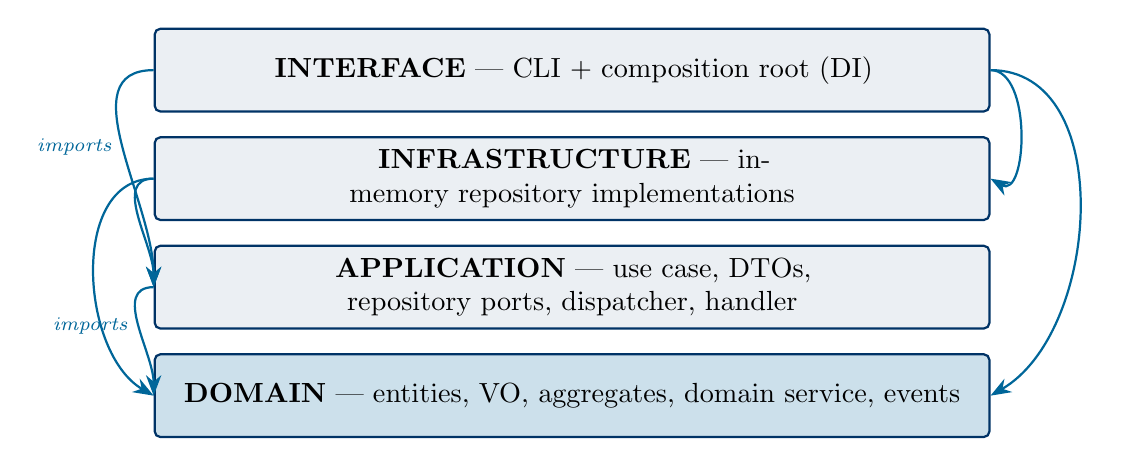
\begin{tikzpicture}[
      ylayer/.style={draw=primary, thick, rounded corners=2pt, align=center,
        minimum width=10.6cm},
      imp/.style={-{Stealth[length=2.6mm]}, thick, color=accent},
      lbl/.style={font=\scriptsize\itshape\color{gray}},
    ]
    \node[ylayer, text width=9.9cm, minimum height=1.05cm, fill=primary!8]
      (interface) { \textbf{INTERFACE} --- CLI + composition root (DI) };
    \node[ylayer, text width=9.9cm, minimum height=1.05cm, fill=primary!8,
      below=0.30cm of interface]
      (infra) { \textbf{INFRASTRUCTURE} --- in-memory repository implementations };
    \node[ylayer, text width=9.9cm, minimum height=1.05cm, fill=primary!8,
      below=0.30cm of infra]
      (app) { \textbf{APPLICATION} --- use case, DTOs, repository ports, dispatcher, handler };
    \node[ylayer, text width=9.9cm, minimum height=1.05cm, fill=accent!20,
      below=0.30cm of app]
      (domain) { \textbf{DOMAIN} --- entities, VO, aggregates, domain service, events };

    \draw[imp] (interface.west) to[out=180,in=90] node[lbl,left] {imports} (app.west);
    \draw[imp] (app.west) to[out=180,in=90] node[lbl,left] {imports} (domain.west);
    \draw[imp] (infra.west) to[out=180,in=90] (app.west);
    \draw[imp] (infra.west) to[out=180,in=150] (domain.west);
    \draw[imp] (interface.east) to[out=0,in=330] (infra.east);
    \draw[imp] (interface.east) to[out=0,in=30] (domain.east);
  \end{tikzpicture}

  \vspace{0.12cm}
  {\scriptsize Dependencies point inward only --- verified by
  \code{scripts/check\_dependencies.py}: ``OK: all imports point inward.''.

  \texttt{Domain $\rightarrow$ (nothing) \;\;
  Application $\rightarrow$ Domain \;\;
  Infrastructure $\rightarrow$ Application, Domain \;\;
  Interface $\rightarrow$ Application, Infrastructure, Domain}}
\end{frame}

% =====================================================================
%  SLIDE 9 - Application service, DTOs, DI (CORRECTED)
% =====================================================================
\begin{frame}{Application Service, DTOs \& Dependency Injection}
  \begin{columns}[t]
    \begin{column}{0.4\textwidth}
      \begin{block}{ConfirmReservationService (coordinates only)}
        \scriptsize
        \begin{enumerate}
          \item Receive \code{ConfirmReservationInput}
          \item Retrieve Reservation --- BR6
          \item Retrieve the related Show
          \item Check eligibility --- BR4
          \item \code{reservation.confirm()} --- BR2
          \item Dispatch \code{ReservationConfirmed} --- BR5; handler calls
                \code{Show.reserve\_seat()} --- BR3
          \item Save the Reservation (handler saved the Show)
          \item Return \code{ConfirmReservationOutput}
        \end{enumerate}
      \end{block}
    \end{column}
    \begin{column}{0.6\textwidth}
      \begin{block}{DTOs}
        \scriptsize
        \begin{itemize}
          \item \textbf{Input:} \code{ConfirmReservationInput(reservation\_id)}
          \item \textbf{Output:} \code{ConfirmReservationOutput}
                \code{(reservation\_id, status, success, message)}
        \end{itemize}
      \end{block}
      \begin{block}{Dependency Injection (constructor)}
        \scriptsize Injected from outside:
        \code{ReservationRepository} \code{ShowRepository}
        \code{ReservationEligibilityService} \code{EventDispatcher}
        (with \code{ReservationConfirmedHandler} registered) +
        \code{clock} (fixed in tests).\\
        {\scriptsize\itshape cli.py and the tests supply the in-memory
        implementations; the service depends on abstractions only.}
      \end{block}
    \end{column}
  \end{columns}
\end{frame}

% =====================================================================
%  SLIDE 10 - BR5 domain event flow
% =====================================================================
\begin{frame}{BR5 --- Domain Event Flow}
  \begin{columns}[t]
    \begin{column}{0.34\textwidth}
      \scriptsize
      \textbf{Before the event is raised}
      \begin{itemize}
        \item Reservation is retrieved (BR6)
        \item BR4 eligibility checked
        \item \code{Reservation.confirm()} --- BR2
        \item State: PENDING $\rightarrow$ CONFIRMED
        \item \code{ReservationConfirmed} is raised
      \end{itemize}
      \vspace{0.15cm}
      \textbf{Event data}\\
      \code{reservation\_id}, \code{customer\_id}, \code{show\_id},
      \code{seat\_number}
    \end{column}
    \begin{column}{0.34\textwidth}
      \scriptsize
      \textbf{Flow}
      \begin{enumerate}
        \item Request $\rightarrow$ \code{ConfirmReservationService}
        \item \code{Reservation} (Aggregate A): \code{confirm()}
        \item \code{ReservationConfirmed}
        \item \code{EventDispatcher}: routes by event type
        \item \code{ReservationConfirmedHandler}: load -- call -- save
        \item \code{Show} (Aggregate B): \code{reserve\_seat()}
      \end{enumerate}
    \textbf{Layer Supertype}\\
      \code{DomainEvent} is the supertype of every domain event; the
      dispatcher and any subscriber program against the abstraction.
    \end{column}
    \begin{column}{0.32\textwidth}
      \scriptsize
      \textbf{Aggregate B rule check (BR3)}\\
      A ShowSeat may be allocated to at most one Reservation.
      \begin{itemize}
        \item AVAILABLE $\rightarrow$ RESERVED by R001 \checkmark
        \item RESERVED by R999 $\rightarrow$ by R001 \ding{55}
              $\rightarrow$ \code{SeatAlreadyReserved}
      \end{itemize}
      \textbf{Failure outcome}\\
      If B rejects: ShowSeat unchanged, Reservation not persisted,
      use case returns failure.
    \end{column}
  \end{columns}
\end{frame}

% =====================================================================
%  SLIDE 11 - Automated tests T1-T8
% =====================================================================
\begin{frame}{Automated Tests T1--T8}
  \centering
  \scriptsize
  \begin{tabularx}{\textwidth}{@{}l l X@{}}
    \toprule
    \textbf{Test} & \textbf{Rule} & \textbf{What it checks (expected result)} \\
    \midrule
    \code{T1} & BR1 & Valid/invalid seat numbers; \code{A1}/\code{Z50} OK;
      \code{A0}/\code{A51} rejected (\code{InvalidSeatNumberError}) \\
    \code{T2} & BR2 & PENDING $\rightarrow$ CONFIRMED succeeds; re-confirming raises
      \code{InvalidReservationStateError} \\
    \code{T3} & BR3 & AVAILABLE seat reserved once; same seat again raises
      \code{SeatAlreadyReservedError}; other show / other seat independent \\
    \code{T4} & BR4 & \emph{Boundary:} $<$4 seats OK; exactly 4 rejected; started/now
      show rejected; other show/customer don't count \\
    \code{T5} & BR5 & Confirming raises \code{ReservationConfirmed} with correct
      data; no event on rejection; handler reserves the seat \\
    \code{T6} & BR6 & Missing reservation $\rightarrow$ \code{ReservationNotFoundError};
      existing proceeds; repo returns \code{None} for unknown id \\
    \code{T7} & Main use case & Success: reservation CONFIRMED, seat RESERVED,
      event handled \\
    \code{T8} & Follow-up & Seat already taken $\rightarrow$ fails; reservation stays
      PENDING, show unchanged \\
    \bottomrule
  \end{tabularx}

  \vspace{0.2cm}
  {\scriptsize T1--T6 verify each business rule; T7--T8 verify the complete
  cross-aggregate workflow (success and failure).\\
  \emph{Rejection cases} throughout; \emph{boundary cases}: 4-seat limit (T4),
  seat-number limits (T1). \textbf{28 test functions --- all pass.}}
\end{frame}

% =====================================================================
%  SLIDE 12 - TDD example (CORRECTED, real evidence)
% =====================================================================
\begin{frame}{TDD Example: BR4 (RED $\rightarrow$ GREEN $\rightarrow$ REFACTOR)}
  \begin{columns}[t]
    \begin{column}{0.5\textwidth}
      \scriptsize
      \textbf{Selected test:} \code{test\_t4\_br4\_future\_show\_with\_four\_%
      confirmed\_seats\_is\_rejected} (T4)\\
      \textbf{Business rule:} BR4 cross-concept rule --- eligible only if the
      Show has not started AND the customer holds fewer than four confirmed
      seats for that Show.
      \vspace{0.15cm}

      \textbf{1. RED --- write the test first}
      \begin{itemize}
        \item Customer \code{C001} already holds exactly four seated
              reservations in \code{S001}
        \item Attempt: \code{check\_eligibility()} for a new reservation
        \item Expected: \code{ReservationNotEligibleError}
        \item Temporarily disabled the four-seat limit in
              \code{check\_eligibility()} (\code{if False:})
        \item Result: \textbf{TEST FAILED} ---
              ``DID NOT RAISE ReservationNotEligibleError''
      \end{itemize}
    \end{column}
    \begin{column}{0.5\textwidth}
      \scriptsize
      \textbf{2. GREEN --- minimum behaviour}
      \begin{itemize}
        \item Rule restored in \code{ReservationEligibilityService}: reject
              when \code{show.confirmed\_seat\_count\_for(customer) >= 4}
        \item Result: \textbf{TEST PASSED}; all 7 BR4 tests pass
      \end{itemize}

      \textbf{3. REFACTOR --- improve without changing behaviour}
      \begin{itemize}
        \item Keep BR4 in the stateless Domain Service (spans two aggregates)
        \item No repository: the \code{Show} aggregate owns its seat count
        \item Re-run all tests: \textbf{T1--T8 PASS}
      \end{itemize}

      \begin{block}{Evidence (in repo)}
        \scriptsize \code{evidence/br4\_rule\_verification\_red.txt}
        (1 failed, 6 passed) and \code{evidence/test\_results\_green.txt}
        (28 passed, 0 failed).
      \end{block}
    \end{column}
  \end{columns}
  {\scriptsize\itshape \centering
  The test defined the required behaviour before implementation; the domain
  code was then written only to satisfy that behaviour and refactored without
  breaking it.}
\end{frame}

% =====================================================================
%  SLIDE 13 - Main use case walkthrough (CORRECTED: A1 demo data)
% =====================================================================
\begin{frame}{Main Use Case Walkthrough}
  \begin{columns}[t]
    \begin{column}{0.48\textwidth}
      \scriptsize
      \textbf{Initial state (demo seed)}\\
      Reservation \code{R001}, customer \code{C001}, show \code{S001},
      seat \code{A1}, status PENDING.\\
      Show \code{S001}: start time future, seat \code{A1} AVAILABLE.
      \vspace{0.12cm}

      \textbf{Execution flow}
      \begin{enumerate}
        \item \code{ConfirmReservationInput("R001")}
        \item \code{ConfirmReservationService} coordinates
        \item \code{ReservationRepository.get\_by\_id("R001")} --- exists (BR6)
        \item \code{ShowRepository.get\_by\_id("S001")}
        \item \code{ReservationEligibilityService}: show not started + below
              limit $\rightarrow$ \emph{Eligible} (BR4)
      \end{enumerate}
    \end{column}
    \begin{column}{0.52\textwidth}
      \scriptsize
      \begin{enumerate}\setcounter{enumi}{5}
        \item \code{Reservation.confirm()}: PENDING $\rightarrow$ CONFIRMED (BR2)
        \item \code{ReservationConfirmed} raised (event data: R001, C001,
              S001, A1)
        \item \code{ReservationConfirmedHandler} loads \code{S001}, requests
              \code{Show.reserve\_seat(A1, R001, C001)}
        \item \code{Show}: A1 AVAILABLE $\rightarrow$ RESERVED by R001 (BR3)
        \item Persistence: updated Reservation and Show saved
        \item \code{ConfirmReservationOutput}: \code{success=True},
              \code{status=CONFIRMED}, ``Reservation confirmed and seat
              reserved''
      \end{enumerate}
      \vspace{0.1cm}
      {\scriptsize\itshape CLI: \code{python -m src.interface.cli R001}
      $\rightarrow$ ``R001: CONFIRMED - Reservation confirmed and seat reserved''.}
    \end{column}
  \end{columns}
\end{frame}

% =====================================================================
%  SLIDE 14 - Design choice changed
% =====================================================================
\begin{frame}{Design Choices Changed}
  \begin{columns}[t]
    \begin{column}{0.5\textwidth}
      \begin{block}{Change 1: ShowSeat $\rightarrow$ child of Show}
        \scriptsize
        \begin{itemize}
          \item \textbf{Initial:} ShowSeat treated as an aggregate root
          \item \textbf{Problem:} seat availability only makes sense inside a
                specific Show; BR3 protects the whole seat inventory
          \item \textbf{Final:} Show is the root; ShowSeat is a child entity
          \item \textbf{Benefit:} one clear enforcement point for BR3;
                \code{ShowSeat.\_reserve()} cannot be called from outside
        \end{itemize}
      \end{block}
    \end{column}
    \begin{column}{0.5\textwidth}
      \begin{block}{Change 2: BR4 decided without a repository}
        \scriptsize
        \begin{itemize}
          \item \textbf{Initial:} eligibility service called
                \code{count\_confirmed\_seats()} on the repository
          \item \textbf{Problem:} domain reached into persistence
          \item \textbf{Final:} the Show answers
                \code{confirmed\_seat\_count\_for(customer)}; the service is
                stateless with zero collaborators
          \item \textbf{Benefit:} domain imports nothing; dependencies point
                fully inward
        \end{itemize}
      \end{block}
    \end{column}
  \end{columns}
  {\scriptsize Deeper domain analysis showed Show --- not ShowSeat --- is the
  correct consistency boundary, and that BR4 belongs entirely inside the domain.}
\end{frame}

% =====================================================================
%  SLIDE 15 - Traceability and conclusion
% =====================================================================
\begin{frame}{Traceability and Conclusion}
  \centering
  \scriptsize
  \begin{tabularx}{\textwidth}{@{}l X l X@{}}
    \toprule
    \textbf{Rule} & \textbf{Design} & \textbf{Test} & \textbf{Result} \\
    \midrule
    BR1 & \code{SeatNumber} Value Object & \code{T1} & PASS \\
    BR2 & \code{Reservation.confirm()} Aggregate Root & \code{T2} & PASS \\
    BR3 & \code{Show.reserve\_seat()} Aggregate Root & \code{T3} & RED + PASS \\
    BR4 & \code{ReservationEligibilityService} Domain Service & \code{T4} & RED + PASS \\
    BR5 & \code{ReservationConfirmed} + Handler & \code{T5}/\code{T7} & PASS \\
    BR6 & \code{ReservationRepository} + App Service & \code{T6} & PASS \\
    Main use case & \code{ConfirmReservationService} & \code{T7} & PASS \\
    Follow-up & Show rejects allocation; nothing saved & \code{T8} & PASS \\
    \bottomrule
  \end{tabularx}

  \vspace{0.2cm}
  \begin{columns}
    \begin{column}{0.7\textwidth}
      {\scriptsize \textbf{Conclusion.} Six business rules shaped the domain
      model, aggregate boundaries, application workflow, architecture and
      tests. Each rule has a clear owner, implementation point and test
      evidence. Solution is small, traceable and easy to defend.}
    \end{column}
    \begin{column}{0.3\textwidth}
      {\scriptsize \textbf{References.}\\
      Evans (2015); Martin (2012); Fowler;
      Microsoft DDD Guidance.}
    \end{column}
  \end{columns}
\end{frame}

\end{document}